\documentclass[10pt]{standalone}
\usepackage{amsmath}
\usepackage{pgf,tikz}
\usepackage{mathrsfs}
\usetikzlibrary{arrows}
\pagestyle{empty}
\usetikzlibrary{decorations.text}
\begin{document}
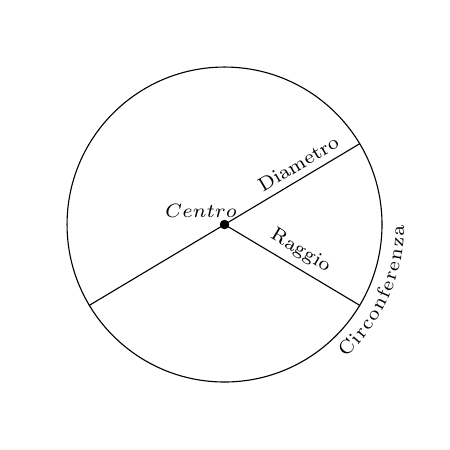
\begin{tikzpicture}[line cap=round,line join=round,>=triangle 45,x=1.0cm,y=1.0cm]
\clip(-2.5,-2.5) rectangle (2.5,2.5);
 

\begin{scriptsize}
 \path[draw, 
postaction={decorate,decoration={%
		text={Circonferenza}, 
		text along path,
		text align=right,
		raise=-8pt,
}}
]
(0,0) circle [radius=2cm];

\draw (0.,0.)-- (1.716724496302083,-1.0260882046863027) node [pos=0.5, sloped, above] {Raggio};
\draw (-1.716724496302083,-1.0260882046863027)-- (1.716724496302083,1.0260882046863027) node [pos=0.8, sloped, above] {Diametro};
\draw [fill=black] (0.,0.) circle (1.5pt);

\draw[color=black] (-0.3,0.17) node {$Centro$};
%\draw[color=black] (-0.94,1.47) node {$c$};
%\draw[color=black] (1.08,0.41) node {$r$};
\end{scriptsize}
\end{tikzpicture}
\end{document}